\documentclass[a4paper]{article}

\def\npart {IB}
\def\nterm {Michaelmas}
\def\nyear {2015}
\def\nlecturer {J. M. Evans}
\def\ncourse {Quantum Mechanics}
\def\nnotready {}

% Imports
\ifx \nextra \undefined
  \usepackage[pdftex,
    hidelinks,
    pdfauthor={Dexter Chua},
    pdfsubject={Cambridge Maths Notes: Part \npart\ - \ncourse},
    pdftitle={Part \npart\ - \ncourse},
  pdfkeywords={Cambridge Mathematics Maths Math \npart\ \nterm\ \nyear\ \ncourse}]{hyperref}
  \title{Part \npart\ - \ncourse}
\else
  \usepackage[pdftex,
    hidelinks,
    pdfauthor={Dexter Chua},
    pdfsubject={Cambridge Maths Notes: Part \npart\ - \ncourse\ (\nextra)},
    pdftitle={Part \npart\ - \ncourse\ (\nextra)},
  pdfkeywords={Cambridge Mathematics Maths Math \npart\ \nterm\ \nyear\ \ncourse\ \nextra}]{hyperref}

  \title{Part \npart\ - \ncourse \\ {\Large \nextra}}
\fi

\author{Lectured by \nlecturer \\\small Notes taken by Dexter Chua}
\date{\nterm\ \nyear}

\usepackage{alltt}
\usepackage{amsfonts}
\usepackage{amsmath}
\usepackage{amssymb}
\usepackage{amsthm}
\usepackage{booktabs}
\usepackage{caption}
\usepackage{enumitem}
\usepackage{fancyhdr}
\usepackage{graphicx}
\usepackage{mathtools}
\usepackage{microtype}
\usepackage{multirow}
\usepackage{pdflscape}
\usepackage{pgfplots}
\usepackage{siunitx}
\usepackage{tabularx}
\usepackage{tikz}
\usepackage{tkz-euclide}
\usepackage[normalem]{ulem}
\usepackage[all]{xy}

\pgfplotsset{compat=1.12}

\pagestyle{fancyplain}
\lhead{\emph{\nouppercase{\leftmark}}}
\ifx \nextra \undefined
  \rhead{
    \ifnum\thepage=1
    \else
      \npart\ \ncourse
    \fi}
\else
  \rhead{
    \ifnum\thepage=1
    \else
      \npart\ \ncourse\ (\nextra)
    \fi}
\fi
\usetikzlibrary{arrows}
\usetikzlibrary{decorations.markings}
\usetikzlibrary{decorations.pathmorphing}
\usetikzlibrary{positioning}
\usetikzlibrary{fadings}
\usetikzlibrary{intersections}
\usetikzlibrary{cd}

\newcommand*{\Cdot}{\raisebox{-0.25ex}{\scalebox{1.5}{$\cdot$}}}
\newcommand {\pd}[2][ ]{
  \ifx #1 { }
    \frac{\partial}{\partial #2}
  \else
    \frac{\partial^{#1}}{\partial #2^{#1}}
  \fi
}

% Theorems
\theoremstyle{definition}
\newtheorem*{aim}{Aim}
\newtheorem*{axiom}{Axiom}
\newtheorem*{claim}{Claim}
\newtheorem*{cor}{Corollary}
\newtheorem*{defi}{Definition}
\newtheorem*{eg}{Example}
\newtheorem*{fact}{Fact}
\newtheorem*{law}{Law}
\newtheorem*{lemma}{Lemma}
\newtheorem*{notation}{Notation}
\newtheorem*{prop}{Proposition}
\newtheorem*{thm}{Theorem}

\renewcommand{\labelitemi}{--}
\renewcommand{\labelitemii}{$\circ$}
\renewcommand{\labelenumi}{(\roman{*})}

\let\stdsection\section
\renewcommand\section{\newpage\stdsection}

% Strike through
\def\st{\bgroup \ULdepth=-.55ex \ULset}

% Maths symbols
\newcommand{\bra}{\langle}
\newcommand{\ket}{\rangle}

\newcommand{\N}{\mathbb{N}}
\newcommand{\Z}{\mathbb{Z}}
\newcommand{\Q}{\mathbb{Q}}
\renewcommand{\H}{\mathbb{H}}
\newcommand{\R}{\mathbb{R}}
\newcommand{\C}{\mathbb{C}}
\newcommand{\Prob}{\mathbb{P}}
\renewcommand{\P}{\mathbb{P}}
\newcommand{\E}{\mathbb{E}}
\newcommand{\F}{\mathbb{F}}
\newcommand{\cU}{\mathcal{U}}
\newcommand{\RP}{\mathbb{RP}}
\newcommand{\CP}{\mathbb{CP}}

\newcommand{\ph}{\,\cdot\,}

\DeclareMathOperator{\sech}{sech}
\DeclareMathOperator{\cosech}{cosech}
\DeclareMathOperator{\cosec}{cosec}

\DeclareMathOperator{\covol}{covol}
\DeclareMathOperator{\vol}{vol}

\let\Im\relax
\let\Re\relax
\DeclareMathOperator{\Im}{Im}
\DeclareMathOperator{\Re}{Re}
\DeclareMathOperator{\im}{im}
\DeclareMathOperator{\image}{image}
\DeclareMathOperator{\Ann}{Ann}

\DeclareMathOperator*{\res}{res}
\DeclareMathOperator{\Res}{Res}
\DeclareMathOperator{\Ind}{Ind}

\DeclareMathOperator{\tr}{tr}
\DeclareMathOperator{\diag}{diag}
\DeclareMathOperator{\rank}{rank}
\DeclareMathOperator{\card}{card}
\DeclareMathOperator{\spn}{span}
\DeclareMathOperator{\adj}{adj}

\DeclareMathOperator{\erf}{erf}
\DeclareMathOperator{\erfc}{erfc}

\DeclareMathOperator{\ord}{ord}
\DeclareMathOperator{\Sym}{Sym}

\DeclareMathOperator{\sgn}{sgn}
\DeclareMathOperator{\orb}{orb}
\DeclareMathOperator{\stab}{stab}
\DeclareMathOperator{\ccl}{ccl}

\DeclareMathOperator{\lcm}{lcm}
\DeclareMathOperator{\hcf}{hcf}

\DeclareMathOperator{\Int}{Int}
\DeclareMathOperator{\id}{id}

\DeclareMathOperator{\betaD}{beta}
\DeclareMathOperator{\gammaD}{gamma}
\DeclareMathOperator{\Poisson}{Poisson}
\DeclareMathOperator{\binomial}{binomial}
\DeclareMathOperator{\multinomial}{multinomial}
\DeclareMathOperator{\Bernoulli}{Bernoulli}
\DeclareMathOperator{\like}{like}

\DeclareMathOperator{\var}{var}
\DeclareMathOperator{\cov}{cov}
\DeclareMathOperator{\bias}{bias}
\DeclareMathOperator{\mse}{mse}
\DeclareMathOperator{\corr}{corr}

\DeclareMathOperator{\otp}{otp}
\DeclareMathOperator{\dom}{dom}

\DeclareMathOperator{\Root}{Root}
\DeclareMathOperator{\supp}{supp}
\DeclareMathOperator{\rel}{rel}
\DeclareMathOperator{\Hom}{Hom}
\DeclareMathOperator{\Aut}{Aut}
\DeclareMathOperator{\Gal}{Gal}
\DeclareMathOperator{\Mat}{Mat}
\DeclareMathOperator{\End}{End}
\DeclareMathOperator{\Char}{char}
\DeclareMathOperator{\ev}{ev}
\DeclareMathOperator{\St}{St}
\DeclareMathOperator{\Lk}{Lk}
\DeclareMathOperator{\disc}{disc}
\DeclareMathOperator{\Isom}{Isom}
\DeclareMathOperator{\length}{length}
\DeclareMathOperator{\energy}{energy}
\DeclareMathOperator{\area}{area}
\DeclareMathOperator{\Syl}{Syl}
\DeclareMathOperator{\cl}{cl}
\DeclareMathOperator{\fix}{fix}

\newcommand{\GL}{\mathrm{GL}}
\newcommand{\SL}{\mathrm{SL}}
\newcommand{\PGL}{\mathrm{PGL}}
\newcommand{\PSL}{\mathrm{PSL}}
\newcommand{\PSU}{\mathrm{PSU}}
\newcommand{\Or}{\mathrm{O}}
\newcommand{\SO}{\mathrm{SO}}
\newcommand{\U}{\mathrm{U}}
\newcommand{\SU}{\mathrm{SU}}

\renewcommand{\d}{\mathrm{d}}
\newcommand{\D}{\mathrm{D}}

\tikzset{->/.style = {decoration={markings,
                                  mark=at position 1 with {\arrow[scale=2]{latex'}}},
                      postaction={decorate}}}
\tikzset{<-/.style = {decoration={markings,
                                  mark=at position 0 with {\arrowreversed[scale=2]{latex'}}},
                      postaction={decorate}}}
\tikzset{<->/.style = {decoration={markings,
                                   mark=at position 0 with {\arrowreversed[scale=2]{latex'}},
                                   mark=at position 1 with {\arrow[scale=2]{latex'}}},
                       postaction={decorate}}}
\tikzset{->-/.style = {decoration={markings,
                                   mark=at position #1 with {\arrow[scale=2]{latex'}}},
                       postaction={decorate}}}
\tikzset{-<-/.style = {decoration={markings,
                                   mark=at position #1 with {\arrowreversed[scale=2]{latex'}}},
                       postaction={decorate}}}

\tikzset{circ/.style = {fill, circle, inner sep = 0, minimum size = 3}}
\tikzset{mstate/.style={circle, draw, blue, text=black, minimum width=0.7cm}}

\definecolor{mblue}{rgb}{0.2, 0.3, 0.8}
\definecolor{morange}{rgb}{1, 0.5, 0}
\definecolor{mgreen}{rgb}{0.1, 0.4, 0.2}
\definecolor{mred}{rgb}{0.5, 0, 0}

\def\drawcirculararc(#1,#2)(#3,#4)(#5,#6){%
    \pgfmathsetmacro\cA{(#1*#1+#2*#2-#3*#3-#4*#4)/2}%
    \pgfmathsetmacro\cB{(#1*#1+#2*#2-#5*#5-#6*#6)/2}%
    \pgfmathsetmacro\cy{(\cB*(#1-#3)-\cA*(#1-#5))/%
                        ((#2-#6)*(#1-#3)-(#2-#4)*(#1-#5))}%
    \pgfmathsetmacro\cx{(\cA-\cy*(#2-#4))/(#1-#3)}%
    \pgfmathsetmacro\cr{sqrt((#1-\cx)*(#1-\cx)+(#2-\cy)*(#2-\cy))}%
    \pgfmathsetmacro\cA{atan2(#2-\cy,#1-\cx)}%
    \pgfmathsetmacro\cB{atan2(#6-\cy,#5-\cx)}%
    \pgfmathparse{\cB<\cA}%
    \ifnum\pgfmathresult=1
        \pgfmathsetmacro\cB{\cB+360}%
    \fi
    \draw (#1,#2) arc (\cA:\cB:\cr);%
}
\newcommand\getCoord[3]{\newdimen{#1}\newdimen{#2}\pgfextractx{#1}{\pgfpointanchor{#3}{center}}\pgfextracty{#2}{\pgfpointanchor{#3}{center}}}

\def\Xint#1{\mathchoice
   {\XXint\displaystyle\textstyle{#1}}%
   {\XXint\textstyle\scriptstyle{#1}}%
   {\XXint\scriptstyle\scriptscriptstyle{#1}}%
   {\XXint\scriptscriptstyle\scriptscriptstyle{#1}}%
   \!\int}
\def\XXint#1#2#3{{\setbox0=\hbox{$#1{#2#3}{\int}$}
     \vcenter{\hbox{$#2#3$}}\kern-.5\wd0}}
\def\ddashint{\Xint=}
\def\dashint{\Xint-}


\begin{document}
\maketitle
{\small
\noindent\textbf{Physical background}\\
Photoelectric effect. Electrons in atoms and line spectra. Particle diffraction.\hspace*{\fill} [1]

\vspace{10pt}
\noindent\textbf{Schr\"odinger equation and solutions}\\
De Broglie waves. Schr\"odinger equation. Superposition principle. Probability interpretation, density and current.\hspace*{\fill} [2]

\vspace{5pt}
\noindent Stationary states. Free particle, Gaussian wave packet. Motion in 1-dimensional potentials, parity. Potential step, square well and barrier. Harmonic oscillator.\hspace*{\fill} [4]

\vspace{10pt}
\noindent\textbf{Observables and expectation values}\\
Position and momentum operators and expectation values. Canonical commutation relations. Uncertainty principle.\hspace*{\fill} [2]

\vspace{5pt}
\noindent Observables and Hermitian operators. Eigenvalues and eigenfunctions. Formula for expectation value.\hspace*{\fill} [2]

\vspace{10pt}
\noindent\textbf{Hydrogen atom}\\
Spherically symmetric wave functions for spherical well and hydrogen atom.

\vspace{5pt}
\noindent Orbital angular momentum operators. General solution of hydrogen atom.\hspace*{\fill} [5]
}

\tableofcontents
\setcounter{section}{-1}
\section{Introduction}
Quantum mechanics (QM) is a radical generalization of classical physics. Profound new features of quantum mechanics include
\begin{enumerate}
  \item \emph{Quantisation} - Quantities such as energy are often restricted to a discrete set of values, or appear in definite amounts , called \emph{quanta}.
  \item \emph{Wave-particle duality} - Classical concepts of particles and waves become merged in quantum mechanics. They are different aspects of a single entity. So an electron will no longer be thought of a ``particle'' but an entity that has properties of both particles and waves.
  \item Probability and uncertainty - Predictions in quantum mechanics involve probability in a fundamental way. This probability does not arise from our lack of knowledge of the system, but is a genuine uncertainty in reality. In particular, there are limits to what we can ask about a physical system, even in principle. For example, the Heisenberg Uncertainty Relation entails that we cannot accurately know the position \emph{and} momentum of a particle.
\end{enumerate}
Quantum mechanics also involves a new fundamental constant $h$ or $\hbar = \frac{h}{2\pi}$. The dimension of this is $[h] = ML^2T^{-1} = [\text{energy}]\times [\text{time}] = [\text{position}] \times [\text{momentum}]$.

We can think of this constant as representing the ``strength'' of quantum effects. Despite having these new profound features, we expect to recover classical physics when we take the limit $\hbar \to 0$.

Historically, there are a few experiments that led to the development of quantum mechanics.
\subsection{Light quanta}
In quantum mechanics, light (or electromagnetic waves) consists of quanta called photons. We can think of them as waves that come in discrete ``packets'' that behave like particles.

In particular, photons behave like particles with energy $E = h \nu = \hbar \omega$, where $\nu$ is the frequency and $\omega = 2\pi \nu$ is the angular frequency. However, we usually don't care about $\nu$ and just call $\omega$ the frequency.

Similarly, the momentum is given by $p = h/\lambda = \hbar k$, where $\lambda$ is the wavelength and $k = 2\pi/\lambda$ is the wave number.

For electromagnetic waves, the speed is $c = \omega/k = \nu\lambda$. This is consistent with the fact that photons are massless particles, since we have
\[
  E = cp,
\]
as entailed by special relativity.

Historically, Planck used the concept of quanta and the energy-frequency relation to derive the spectrum of black body of ``black-body'' radiation that is consistent with experimental results. However, they were not yet sure that light indeed come in quanta. It could have just been a mathematical trick to derive the desired result.

The physical reality of photons was clarified by Einstein in explaining the \emph{photo-electric effect}.

When we shine some light (or electromagnetic radiation $\gamma$) of frequency $\omega$ onto certain metals, this can cause an emission of electrons ($e$). We can measure the maximum kinetic energy $K$ of these electrons.
\begin{center}
  \begin{tikzpicture}
    \draw (-2, 0) -- (2, 0);
    \draw [decorate, decoration={snake}] (-2, 2) -- (0, 0) node [pos = 0.5, anchor=south west] {$\gamma$}; % make curly
    \draw [->] (0, 0) -- (2, 2) node [right] {$e$};
  \end{tikzpicture}
\end{center}
Experiments show that
\begin{enumerate}
  \item The number of electrons emitted depends on the intensity (brightness) of the light, but not the frequency.
  \item The kinetic energy $K$ depends only (linearly) on the frequency but not the intensity.
  \item For $\omega < \omega_0$ (for some critical value $\omega_0$), \emph{no} electrons are emitted at all.
\end{enumerate}
This is hard to understand classically, but is exactly as expected if each electron emitted is due to the impact with a single photon. If $W$ is the energy required to liberate an electron, then we would expect $K = \hbar \omega - W$ by the conservation of energy. We will have no emission if $\omega < \omega_0 = W/\hbar$.

\subsection{Bohr model of the atom}
When we heat atoms up to make them emit light; or shine light at atoms so that they absorb light, we will find that light is emitted and absorbed at very specific frequencies, known as the emission and absorption spectra. This suggests that the inner structure of atoms is discrete.

However, in the classical model, the simplest atom, the hydrogen, consists of an electron with charge $-e$ and mass $m$, orbiting a proton of charge $+e$ and mas $m_p \gg m$ fixed at the origin.

The potential energy is
\[
  V(r) = -\frac{e^2}{4\pi\varepsilon_0}\frac{1}{r}.
\]
This implies that the angular momentum $\mathbf{L}$ is constant, and the energy $E = \frac{1}{2}mv^2 + V(r)$ is constant.

This is not a very satisfactory model for the atom. First of all, it cannot explain the discrete emission and absorption spectra. More importantly, while this model seems like a mini solar system, electromagnetism behave differently from gravitation. To maintain a circular orbit, an acceleration has to be applied onto the electron. Indeed, the force is given by
\[
  F = \frac{mv^2}{r} = \frac{e^2}{4\pi \varepsilon_0}\frac{1}{r^2}.
\]
Accelerating particles emit radiation and lose energy. So according to classical electrodynamics, the electron will just decay into the proton and atoms will implode.

The solution to this problem is to simply declare that this cannot happen. The \emph{Bohr quantization conditions} restricts the classical orbits by saying that the angular momentum can only take values
\[
  L = mrv = n\hbar
\]
for $n = 1, 2, \cdots$. Using these, together with the force equation, we can solve $r$ and $v$ completely for each $n$and obtain
\begin{align*}
  r_n &= \frac{4\pi \varepsilon_0}{me^2}\hbar^2 n^2\\
  v_n &= \frac{e^2}{4\pi \varepsilon_0}\frac{1}{\hbar n}\\
  E_n &= -\frac{1}{2}m\left(\frac{e^2}{4\pi \varepsilon_0 \hbar}\right)^2 \frac{1}{n^2}.
\end{align*}
Now we assume that the electron can make transitions between different energy levels $n$ and $m > n$, accompanied by emission or absorption of a photon of frequency $\omega$ given by
\[
  E = \hbar \omega = E_n - E_m = \frac{1}{2}m \left(\frac{e^2}{4\pi \varepsilon_0 \hbar}\right)^2\left(\frac{1}{n^2} - \frac{1}{m^2}\right).
\]
\begin{center}
  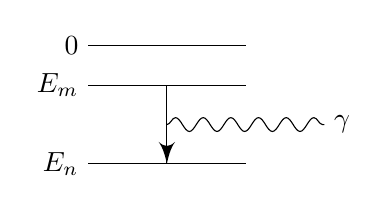
\begin{tikzpicture}
    \draw (-1, 0) node [left] {$0$} -- (1, 0);
    \draw (-1, -0.5) node [left] {$E_m$} -- (1, -0.5);
    \draw (-1, -1.5) node [left] {$E_n$} -- (1, -1.5);
    \draw [->] (0, -0.5) -- (0, -1.5);
    \draw [decorate, decoration={snake}] (0, -1) -- (2, -1) node [right] {$\gamma$};
  \end{tikzpicture}
\end{center}
This model explains a \emph{vast} amount of experimental data. This also gives an estimate of the size of a hydrogen atom:
\[
  r = \left(\frac{4\pi \varepsilon_0}{me^2}\right) \hbar^2 \approx \SI{5.29e-11}{\meter},
\]
known as the \emph{Bohr radius}.

Nevertheless, we would like a better understanding of why angular momentum should be quantized.

\subsection{Matter waves}
The relation
\begin{align*}
  E &= h\nu = \hbar \omega\\
  p &= \frac{h}{\lambda} = \hbar k
\end{align*}
are used to associate particle properties (energy and momentum) to waves. They can also be used the other way round - to associate wave properties (frequency and wave number) to particles. Moreover, these apply to non-relativistic particles such as electrons (as well as relativistic photons). This $\lambda$ is known as the \emph{de Broglie wavelength}. How does this fit in into our existing model?

Recall that the quantization of the Bohr model requires that
\[
  L = rp = n\hbar.
\]
Using the relations above, this is equivalent to requiring that
\[
  n\lambda = 2\pi r.
\]
This requires that the circumference of the orbit is an integer multiple of the wavelength. This is somewhat the condition we need for a standing wave to form on the circumference. This looks promising as an explanation for the quantization relation.

But in reality, do electrons actually behave like waves? If electrons really are waves, then they should exhibit the usual behaviour of waves, such as diffraction and interference.

We can repeat our favorite double-slit experiment on electrons. We have a sinusoidal wave incident on some barrier with narrow openings as shown:
\begin{center}
  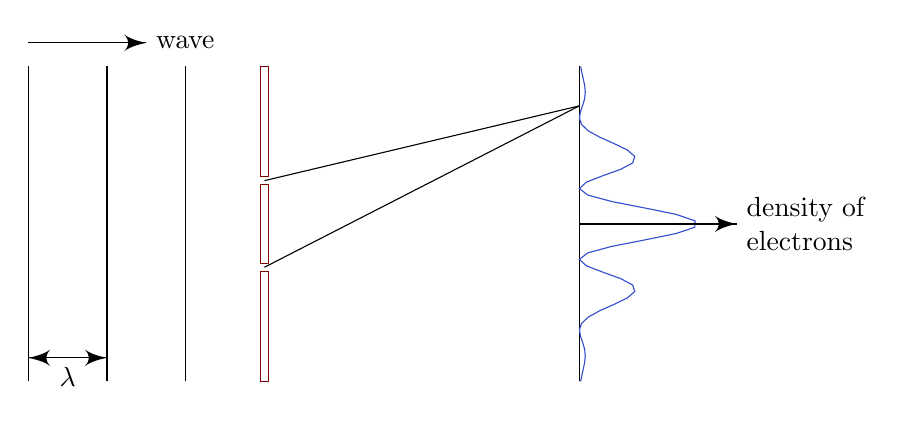
\begin{tikzpicture}
    \draw [mred] (-0.05, -0.5) rectangle (0.05, 0.5);
    \draw [mred] (-0.05, 0.6) rectangle (0.05, 2);
    \draw [mred] (-0.05, -0.6) rectangle (0.05, -2);
    \draw (4, -2) -- (4, 2);

    \foreach \x in {-1, -2, -3} {
      \draw (\x, -2) -- (\x, 2);
    }

    \draw [<->] (-2, -1.7) -- (-3, -1.7) node [below, pos=0.5] {$\lambda$};
    \draw [->] (-3, 2.3) -- (-1.5, 2.3) node [right] {wave};

    \draw (0, 0.55) -- (4, 1.5);
    \draw (0, -0.55) -- (4, 1.5);
    \draw [domain=-2:2,samples=50, mblue] plot ({4 + 1.5 * exp(-\x * \x) * (cos (200 * \x))^2}, \x);
    \draw [->, align=left] (4, 0) -- (6, 0) node [right] {density of\\ electrons};
  \end{tikzpicture}
\end{center}
At different points, Depending on the difference $\delta$ in path length, we may have constructive interference (large amplitude) or destructive interference (no amplitude). In particular, constructive interference occurs if $\delta = n\lambda$, and destructive if $\delta = (n + \frac{1}{2})\lambda$.

Not only does this experiment allow us to verify if something is a wave. We can also figure its wavelength $\lambda$ by experiment.

Practically, the actual experiment for electrons is slightly more complicated. Since the wavelength of an electron is rather small, to obtain the diffraction pattern, we cannot just poke holes in sheets. Instead, we need to use crystals as our diffraction grating. Nevertheless, this shows that electrons do diffract, and the wavelength \emph{is} the de Broglie wavelength.

This also has a conceptual importance. For regular waves, diffraction is something we can make sense of. However, here we are talking about electrons. We know that if we fire many many electrons, the distribution will follow the pattern described above. But what if we just fire a single electron? On \emph{average}, it should still follow the distribution. However, for this individual electron, we cannot know where it will actually land. We can only provide a probability distribution of where it will end up. In quantum mechanics, everything is inherently probabilistic.

As we have seen, quantum mechanics is vastly different from classical mechanics. This is unlike special relativity, where we are just making adjustments to Newtonian mechanics. In fact, in IA Dynamics and Relativity, we just ``derived'' special relativity by assuming the principle of relativity and that the speed of light is independent of the observer. This is not something we can do for quantum mechanics - what we are going to do is just come up with some theory and then show (or claim) that they agree with experiment.

\section{Wavefunctions and the \texorpdfstring{Schr\"odinger}{Schrodinger} equation}
To begin with, we will concentrate on quantum mechanics in one dimension only.

\subsection{Particle state and probability}
Classically, a point particle in 1 dimension has a definitive position $x$ (and momentum $p$) at each time. In quantum mechanics, a particle has a \emph{state} at each time, specified by a complex-valued \emph{wavefunction} $\Psi(x)$.

If $\Psi$ is appropriately normalized, then when we measure the position of a particle, we get a result $x$ with probability density function $|\Psi(x)|^2$, ie. the probability that the position is found in $[x, x + \delta x]$ (for small $\delta x$) is given by $|\Psi(x)|^2 \delta x$. Alternatively, the probability of finding it in $[a, b]$ is given by
\[
  \P(\text{particle position in }[a, b]) = \int_a^b |\Psi(x)|^2 \;\d x.
\]
What do we mean by ``appropriately normalized''? From our equation above, we see that we require
\[
  \int_{-\infty}^\infty |\Psi(x)|^2\;\d x = 1,
\]
since this is the total probability of finding the particle anywhere at all. This the normalization condition required.

\begin{eg}[Gaussian wavefunction]
  We define
  \[
    \Psi(x) = C e^{-\frac{(x - c)^2}{2\alpha}},
  \]
  where $c$ is realm $C$ could be complex.
  \begin{center}
    \begin{tikzpicture}[yscale=1.5]
      \draw (-3, 0) -- (3, 0);
      \draw (0, 1.3) --  (0, 0) node [below] {$c$};
      \draw [domain=-3:3,samples=50, mblue] plot (\x, {exp(-\x * \x)});
    \end{tikzpicture}
  \end{center}
  We have
  \[
    \int_{-\infty}^\infty |\Psi(x)|^2 \;\d x = |C|^2 \int_{-\infty}^{\infty}e^{-\frac{(x - c)^2}{\alpha}} \;\d x = |C|^2 (\alpha \pi)^{\frac{1}{2}} = 1.
  \]
  So for normalization, we need to pick $C = (1/\alpha \pi)^{1/4}$ (up to a multiple of $e^{i\theta}$).

  If $\alpha$ is small, then we have a sharp peak around $x = c$. If $\alpha$ is large, it is more spread out.
\end{eg}
While it is nice to have a normalized wavefunction, it is often inconvenient to deal exclusively with normalized wavefunctions, or else we will have a lot of ugly-looking constants floating all around. As a matter of fact, we can always restore normalization at the end of the calculation. So we often don't bother.

If we do not care about normalization, then for any (non-zero) $\lambda$, $\Psi(x)$ and $\lambda \Psi(x)$ represent the same quantum state (since they give the same probabilities). In practice, we usually refer to either of these as ``the state''.

What we do require, then, is not that the wavefunction is normalized, but \emph{normalizable}, ie.
\[
  \int_{-\infty}^\infty |\Psi(x)|^2 \;\d x < \infty.
\]
A characteristic property of quantum mechanics is that if $\Psi_1(x)$ and $\Psi_2(x)$ are wavefunctions for a particle, then $\Psi_1(x) + \Psi_2 (x)$ is also a possible particle state (ignoring normalization), provided the result is non-zero. This is the principle of superposition, and arises from the fact that the equations of quantum mechanics are linear.
\end{document}
